   
\section{\MakeUppercase{System Architecture and Methodology}}
\subsection{Dataset}
For the successful implementation of the approach, a carefully maintained dataset is required, consisting of wireframe sketches paired with their corresponding \gls{dsl} code. These sketches and codes are fundamental for training the machine learning model to recognize and translate visual designs into functional code. However, a pre-existing dataset containing both wireframe sketches and the associated \gls{dsl} code could not be found. It was determined during the research that no publicly available dataset fully met the specific requirements of the project. As a result, the decision was made to create a custom dataset from scratch. This ensured that the dataset closely aligns with the goals of the project and contains the necessary variety and diversity for effective model training.

\subsubsection{Dataset Generator}
The dataset generator plays a central role in the project, as it is responsible for producing a vast and varied set of training samples that will be used by the model. This generator operates through a structured, multi-step process designed to create the necessary wireframe sketches and their corresponding \gls{dsl} code. The process begins with the random generation of \gls{dsl} code, which specifies the structural elements and layout of a web page. The generated \gls{dsl} code is then compiled into HTML and CSS, which are used to render a visual representation of the web page layout. Once the visual layout is created, the rendered page is analyzed to identify and map out the positions and boundaries of each individual element. These identified positions are crucial for accurately placing the corresponding visual elements in the next phase. In the final step of the process, hand-drawn sketches are placed onto the generated layout at the appropriate positions. These sketches mimic the real-world designs of web pages, but in a simplified, hand-drawn style, closely resembling wireframe designs.This automated process allows for the production of a large number of unique and diverse sketch-\gls{dsl} pairs. Each pair is representative of realistic, real-world web page designs, and the generator ensures that these pairs are varied in structure, complexity, and design style. By utilizing predefined rules and constraints, the dataset generator ensures that the generated layouts are not only realistic but also diverse, capturing the wide range of design possibilities that exist in the real world. With this automated dataset generation process, as many samples as required for training the model can be efficiently generated without relying on manual data collection. This ensures that the model is exposed to a broad set of design styles and can accurately learn to translate wireframe sketches into functional \gls{dsl} code.

\begin{figure}[H]
    \centering
    \includegraphics[width=\textwidth]{images/Dataset Generator.png}\caption{Block Diagram of Data Synthesis}\label{fig:Synthesis}
\end{figure}



    \subsection{Block Diagram}

 \begin{figure}[H]
        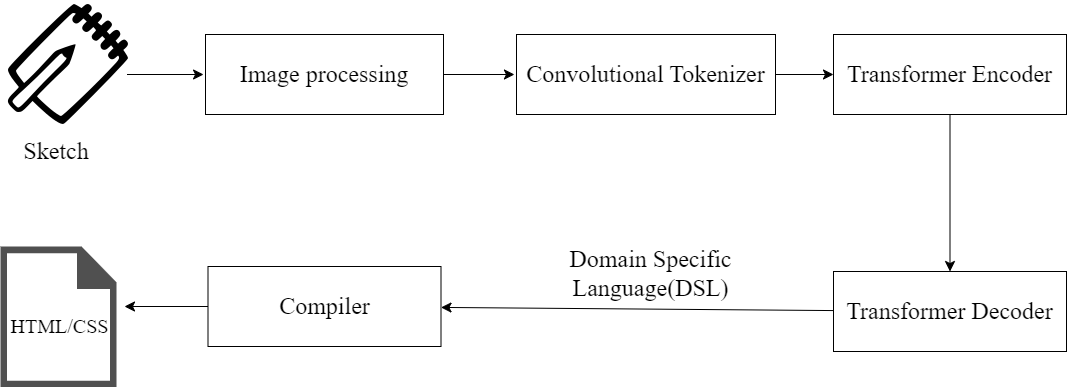
\includegraphics[scale=5]{images/Block Diagram.png}
        \caption{Block Diagram of Working of System}
        \label{fig:block}
    \end{figure}

    \subsection{Working Principle}
    The core principle behind this project is to transform a manually created wireframe sketch of a user interface (UI) into functional HTML code. The process involves several key stages, each aimed at capturing the essential visual components of the sketch and translating them into corresponding HTML elements. The following steps outline the approach taken to achieve this transformation:

    \begin{enumerate}
        \item \textbf{DSL Code Extraction using Transformer Model:}
        
        The first step in the process involves extracting the domain-specific language (\gls{dsl}) code from the input sketch. The sketch, which serves as a visual representation of the UI, is analyzed using a deep learning model, specifically a Transformer model, which has been trained to recognize the structure and components of the design. The Transformer model is particularly useful in understanding the spatial relationships between different UI elements in the sketch. Through a process of visual recognition and feature extraction, the model identifies components such as buttons, text fields, images, and containers, and generates the corresponding \gls{dsl} code. This code is a simplified representation of the layout, defining the structure and properties of each UI element.

        \item \textbf{Compiling DSL Code to HTML Code:}
        Once the \gls{dsl} code has been extracted, the next step is to compile it into HTML code. The generated \gls{dsl} code serves as a blueprint for the layout, and each \gls{dsl} element corresponds to a specific HTML tag or structure. This step involves mapping the \gls{dsl} elements to their respective HTML equivalents, ensuring that the visual design described by the \gls{dsl} is accurately translated into a functional HTML layout. This step may involve additional styling elements, such as CSS for positioning and design tweaks, to ensure the generated HTML code matches the intended appearance of the original sketch. 
        The process in this project has two main steps—first, extracting the DSL code using a Transformer model, and then converting it into HTML code. This is the main idea behind how the system works. It automates the process of turning a simple sketch into functional front-end code, making it much easier for developers to create prototypes quickly.Using \gls{ml} techniques like Transformer models, the system can recognize and understand the layout of the design. After that, it converts it into HTML, making sure the design works well in a web browser. This method speeds up development and helps designers and developers communicate better, as it turns a design concept directly into working code.
    \end{enumerate}
\subsubsection{Image Processing}
Preprocessing is required to translate an image from a camera into an image which can
be fed into the model. Due to the positioning of the camera or lighting conditions the
raw image must be cleaned up before it can be processed.

The main challenges are:
\begin{itemize}
    \item The image may not fill the entire frame, as such the background must be
removed. 
    \item The paper may be skewed or rotated.
    \item The image may contain noise or alterations due to lighting.
\end{itemize}

For solving above challenges:
\begin{itemize}
    \item The paper was detected in the image and cropped. As the requirements stated that the medium must be white, the image was converted to HSV, and threshold filtering was applied to remove all colors except white. This process considerably reduced the background noise. Since the paper contained the sketch in a dark marker, these pixels were filtered out using threshold filtering. To fill the gaps left by the sketch, a large median blur was applied. The edge map was then dilated to close small gaps between the edges. Finally, contour detection was applied, and the largest contour with approximately four sides was identified, as it was assumed the medium was four-sided (e.g., paper or a whiteboard).
    \item Perspective warping was applied to unwrap the four corners of the contour found and map them to an equivalent rectangle, thereby correcting the orientation of the page.
    \item A median blur was applied to the unwrapped cropped image to reduce noise. The edge map was then dilated to close small gaps between lines. The result of the post-processing was an unskewed binary edge map of the sketch, which was subsequently fed into the model for processing.
\end{itemize}

\subsubsection{Convolutional Tokenizer}
A convolutional tokenizer is an important component in neural networks, particularly when working with images. This part of the system processes visual data, applying convolutional layers to detect and capture local patterns and features within an image. Convolutional layers work by scanning the image with small filters, which help identify important features such as edges, textures, or shapes at different scales. After applying these filters, the network often uses pooling layers, which reduce the size of the image while keeping the most relevant information intact. This helps make the process more efficient by focusing on the key aspects of the image.The outcome of these convolutional operations is a set of feature maps, which are essentially condensed representations of the image. These feature maps contain high-level abstractions of what is found in the image, making them easier to analyze and interpret. Once the feature maps are generated, they are reshaped or flattened into a sequence of vectors, which are called tokens. Each token represents a specific part of the image, such as a button, a menu, or a text box in the context of UI design. This sequence of tokens can now be treated as input for sequence models, similar to how natural language processing models work with text. By doing so, the convolutional tokenizer enables the application of advanced techniques, like transformers, to image data, which would otherwise be difficult to process.

\subsubsection{Transformer Model}
The Transformer model is a powerful deep learning architecture widely used for tasks involving sequences of data. Its encoder-decoder structure makes it particularly effective for these tasks. The encoder processes the input sequence, with each token representing a feature of the image, and converts them into continuous representations that capture the essential information. Once the encoder has processed the tokens, the decoder generates an output sequence, which, in this case, is the Domain-Specific Language (DSL) code. The decoder uses the encoded information to produce a sequence of symbols that describe the structure of the image or user interface.The Transformer model is designed with self-attention mechanisms, enabling it to focus on different parts of the input sequence simultaneously. This makes the model efficient at understanding complex relationships in data. The self-attention layers, along with fully connected layers, allow the model to capture the most relevant information from the input, even when the data is spread out or has long-range dependencies.In tasks like image captioning, the input is an image, and the output is a text description of what the image contains. However, in this case, the output is a structural description of the user interface in DSL, which defines the layout and behavior of different UI elements. This allows for the generation of detailed, accurate code that represents the structure of the UI, making it easier to convert sketches into functional front-end code.

    \begin{figure}[H]
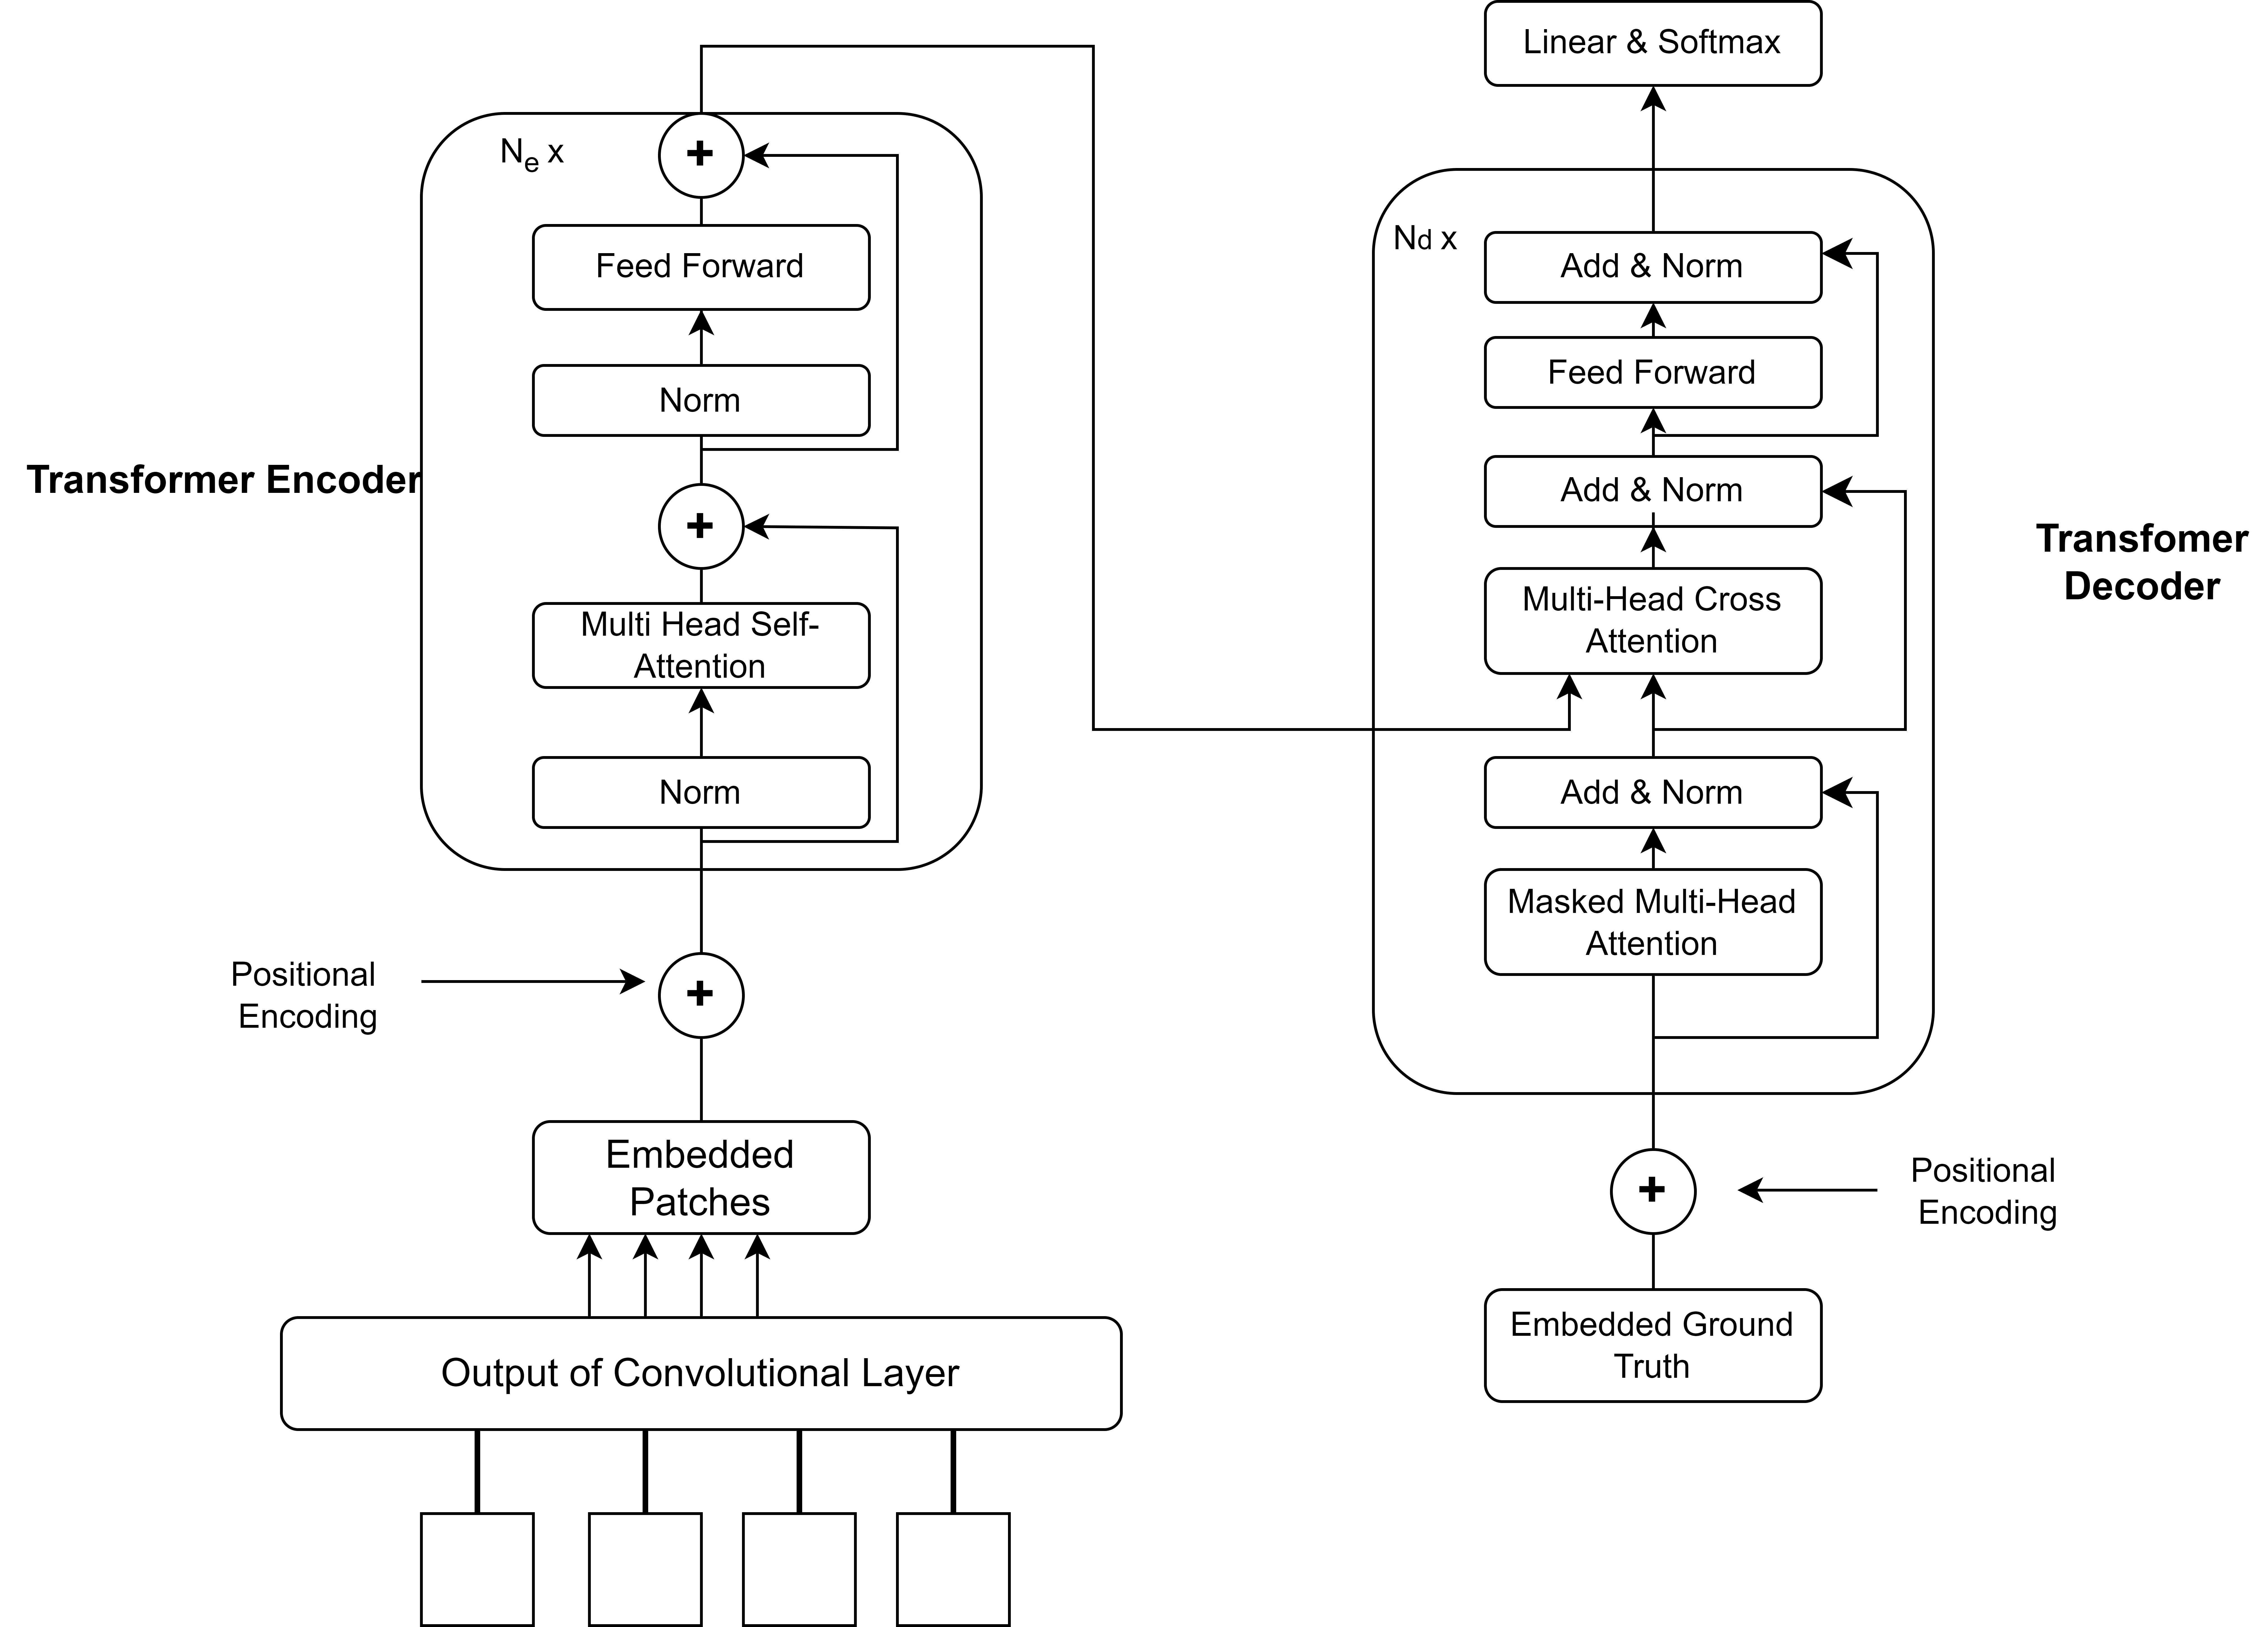
\includegraphics[scale=.7]{images/Transformer.png}
\caption{Block Diagram of Transformer Model}
\label{fig:transfor}
\end{figure}

\textbf{Transformer Encoder}\\
The Transformer encoder is a fundamental part of the Transformer architecture, originally developed for \gls{nlp} tasks but has since been adapted and widely used in various domains, including \gls{cv}. The encoder consists of multiple identical layers, with each layer containing two critical subcomponents: the multi-head self-attention mechanism and the position-wise fully connected feed-forward network. These two subcomponents are designed to handle different aspects of processing the input sequence and help the model learn complex patterns in the data.
The multi-head self-attention mechanism is essential because it enables the model to evaluate the relationships between different elements in the input sequence, regardless of their positions or distance from one another. This is a significant advantage over previous architectures like \gls{rnn}, which processed data sequentially and struggled with long-range dependencies. By using multiple attention heads, the Transformer can simultaneously focus on different parts of the input sequence, capturing diverse relationships and dependencies at different levels of abstraction. This makes it particularly effective for tasks where understanding the context between distant elements in the data is important, such as understanding the layout and structure of an image in computer vision tasks.
The position-wise feed-forward network, which follows the self-attention layer, processes each element independently, applying non-linear transformations to increase the model's capacity to learn more complex functions. This additional step allows the model to better understand intricate patterns within the data. Each position in the sequence is transformed individually, allowing the network to adapt to the unique features of each token. The encoder’s architecture also employs layer normalization and residual connections around each sub-layer, which greatly assist in stabilizing and accelerating the training of deep networks. These techniques make it easier for the model to converge and learn effectively, especially when working with large datasets and complex tasks like image-to-text or sketch-to-code translation.

\textbf{Transformer Decoder}\\
The Transformer decoder, like the encoder, consists of multiple identical layers. In our model, these decoder layers are designed to work with the encoded representations of the image as well as additional information, such as embedded ground truth caption sequences. The decoder is structured similarly to the encoder but with a few key differences to handle the output generation process. Each decoder block contains three main subcomponents: a masked multi-head self-attention sublayer, a multi-head cross-attention sublayer, and a position-wise feed-forward sublayer.
The masked multi-head self-attention mechanism in the decoder ensures that the model can focus on previously generated tokens while predicting the next token in the sequence. This self-attention mechanism is “masked” to prevent the model from attending to future tokens during training, which enforces autoregressive generation. This ensures that the output is produced sequentially, with each new token being generated based on the previous ones, similar to how natural language is generated in a left-to-right manner.
The multi-head cross-attention mechanism allows the decoder to focus on the encoded image embeddings at each time step. By attending to these image representations, the decoder can incorporate relevant visual features into the output sequence. This is particularly useful for tasks such as image captioning or sketch-to-code generation, where the output needs to be grounded in the input image’s content. The cross-attention layer allows the model to align the visual features with the tokens being predicted, ensuring that the generated output is accurate and coherent with the input image.
The position-wise feed-forward sublayer in the decoder operates similarly to the one in the encoder, applying transformations to each token independently. This step adds further capacity to the model, allowing it to better handle the complexity of generating diverse and detailed output sequences. Additionally, positional encodings are added to the embedded ground truth caption sequences to retain the order of the tokens, ensuring that the sequence of words in the output is consistent with the order of the original text.
At each decoding step, the output of the last decoder block is used to predict the next word or symbol in the sequence through a linear transformation, followed by a softmax function. The output dimension of this linear layer corresponds to the size of the vocabulary, allowing the model to predict any word in the vocabulary as the next token in the sequence. This autoregressive process continues until the end of the sequence is reached, and the model has generated a complete output, whether it be a caption, a design description, or another form of structured code.

\textbf{Attention}\\
Attention can be describe as a similarity between the query and key. They take the form:
\begin{equation}
\text{Attention}= \text{similarity}(q, k)
\end{equation}
Where q represents a query and k represents a key. It’s like accessing a database, where
we query the database looking for the information we want. To find the similarity
between queries and keys, dot product is normally used. It provide the value between 0
and 1. If they are different, obtained value is 0 otherwise it is 1. The output is computed
as a weighted sum of the values, where the weight assigned to each value is computed
by a compatibility function of the query with the corresponding key.

\textbf{Self-Attention}\\
In order to identify dependencies and relationships within input sequences, selfattention is a method employed in machine learning, especially in natural language
processing and \gls{cv} applications. By taking care of itself, the model is able
to recognize and assess the relative value of various input sequence components. In
self-attention, vector q, k, v which are actually neural networks (typically linear) have
same input (q(x), k(x), v(x)), then they are self- attending.

\textbf{Scaled Dot-Product Self-Attention}\\
The dimensionality of queries and keys is denoted by \( d_k \), and the dimensionality of values by \( d_v \). The scaled dot-product attention computes the dot product of the queries with the keys, scales the result by the square root of \( d_k \), and applies a softmax function to obtain attention weights. Finally, a weighted multiplication is performed on the data using these attention weights.The complete procedure can be mathematically stated
as follows, where Q, K, and V, represent the keys, values, and queries, correspondingly:
\begin{equation}
\text{Attention}(Q, K, V) = \text{softmax}\left(\frac{QK^T}{\sqrt{d_k}}\right) V
\end{equation}

\textbf{Multi-Head Self-Attention}\\
Instead of performing a single attention function with keys, values and queries, it is
more beneficial to linearly project the queries, keys and values h times with different,
learned linear projections to dk, dk, and dv dimensions, respectively. By performing the
attention function in parallel on each of these projected versions of queries, keys and
values, dv –dimensional values are obtained as output. The ability of attending to input
from several representation subspaces at different points is provided by multi-head
attention to the model.
\begin{equation}
\text{MultiHead}(Q, K, V) = \text{Concat}(\text{head}_1, \dots, \text{head}_h) W^O
\end{equation}
Where \(\text{head}_i = \text{Attention}(QW_i^Q, KW_i^K, VW_i^V)\)

\textbf{Layer Normalization}\\
In deep learning, \gls{ln} is a technique that helps to stabilize the
training process and boost neural network performance. LN separately normalizes each
layer's activations for every feature. This means that the activations are scaled and
shifted to have a standard normal distribution (mean of 0 and variance of 1) after the
mean and variance of the activations are determined independently for each layer.

\textbf{Position Embedding}\\
Position embedding is used to add spatial information to the image data. Since the
model is actually uninformed of the token's spatial relationship, additional information
expressing this relationship can be useful. Usually, this involves assigning tokens
weights derived from two high-frequency sine waves, or using a learned embedding.
This allows the model to understand that these tokens have a positional relationship.
The standard Transformer uses sine and cosine functions of different frequencies: 
\begin{equation}
PE(pos, 2i) = \sin(\frac{pos}{ 10000^{2i}/dmodel})
\end{equation}

\begin{equation}
PE(pos, 2i + 1) = \cos(\frac{pos}{10000^{2i}/dmodel})
\end{equation}
 Where pos denotes the position and i denotes the dimension.

\textbf{Multi-Layer Perceptron}\\
An MLP is a type of feed forward artificial neural network with multiple layers,
including an input layer, one or more hidden layers, and an output layer. It is an
Artificial Neural Network in which all nodes are interconnected with nodes of different
layers. An input layer, an output layer, and one or more hidden layers with several
neurons stacked on top of each other make up a multilayer perceptron. Additionally,
neurons in a Multilayer Perceptron can employ any arbitrary activation function, unlike neurons in a Perceptron, which must have an activation function that enforces a
threshold, such as ReLU or sigmoid

\begin{figure}[H]
    \centering
    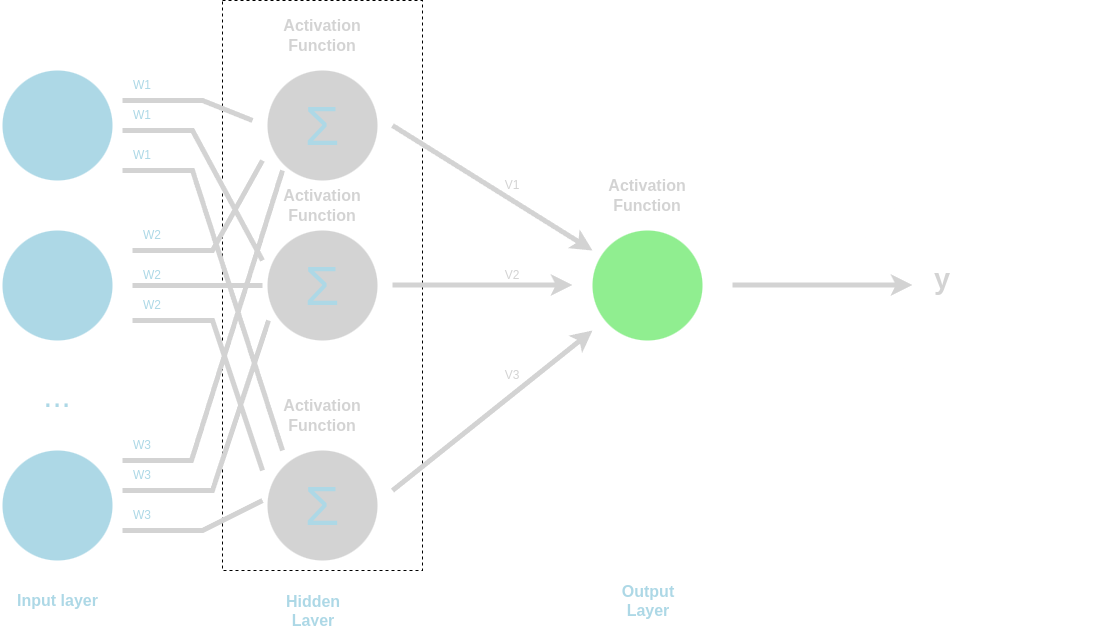
\includegraphics[width=\textwidth]{images/mlp.png}\caption{Multilayer Perceptron}\label{fig:mlp}
\end{figure}







\subsubsection{Domain-Specific Language (DSL)}

A \gls{dsl} is a specialized programming language tailored for a particular task, domain, or set of applications. Unlike general-purpose programming languages such as Python, Java, or C++, which are designed to be versatile and applicable to a wide range of projects, DSLs are focused on a specific problem or field. This specialization allows DSLs to provide more efficient, readable, and expressive solutions within their target domains.
In this project, we have design a lightweight and simple Domain-Specific Language to describe the layout and structure of graphical user interfaces (GUIs). The primary goal of our DSL is to allow easy representation and translation of UI designs into code that can be processed by a machine. In this DSL, elements like buttons, text fields, and images will be categorized based on their position, type, and hierarchical relationship within the layout. This hierarchical structure will ensure that the DSL can effectively represent the various components of a GUI in a way that is both simple and intuitive to understand.
The key advantage of using a DSL for this project is its simplicity. By narrowing the focus to only the essential components needed to describe the UI, the DSL reduces the complexity of the input space, making it easier for the model to process. This simplification also leads to a smaller vocabulary, as fewer tokens are needed to describe the UI elements. A smaller vocabulary helps improve the efficiency of the model, as it reduces the number of possible options that need to be considered during the learning process.
Additionally, to address potential challenges like overfitting and the need for better generalization, we introduce compact convolutional transformers. These models are designed to work efficiently with small datasets by focusing on compact architectures that maintain a balance between performance and model size. Compared to traditional Convolutional Neural Networks (CNNs), compact convolutional transformers are better suited for tasks with limited data, as they have fewer parameters and are less prone to overfitting. This allows the model to learn more robust features from smaller datasets, ensuring better results even when there is limited training data available.
The simplicity and specialized focus of the DSL make it a powerful tool for this project, enabling effective and accurate conversion of sketches into functional code. By using a DSL, we can streamline the entire process of UI design representation, making it easier to translate complex visual concepts into structured code while maintaining a high degree of flexibility and efficiency in the overall system.

    \begin{figure}[H]
        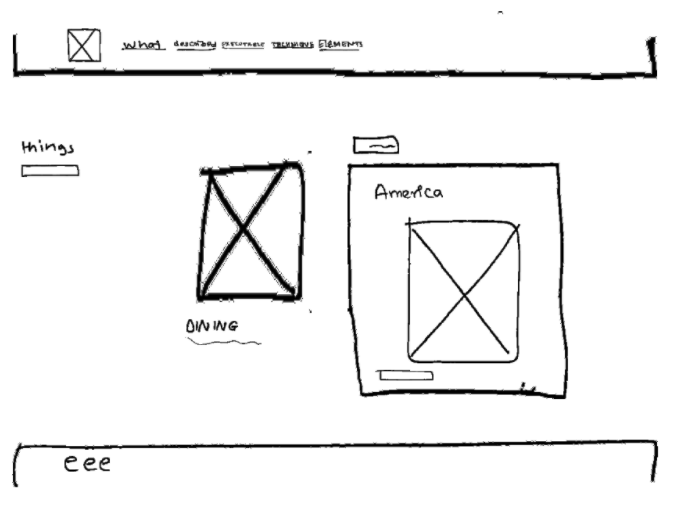
\includegraphics[scale=.6]{images/sample image.png}
        \caption{Sample Input Image}
        \label{fig:lsamp}
    \end{figure}




The sample \gls{dsl} for above image:

% Use the custom command to display the tree structure



\begin{verbatim}
    header{
        flex{
            logodiv{
                image
            }
            nav{
                navlink
                navlink
                navlink
                navlink
                navlink
            }
        }
    }
    container{[
        row{
            div-3{
                text-c
                input
            }
            div-3{
                image
                text
                paragraph
            }
            div-6{
                button
                card{
                    text-c
                    image
                    input
                }
            }
        }
    ]}
    footer{
        text
    }
    \end{verbatim}

    \begin{figure}[H]
        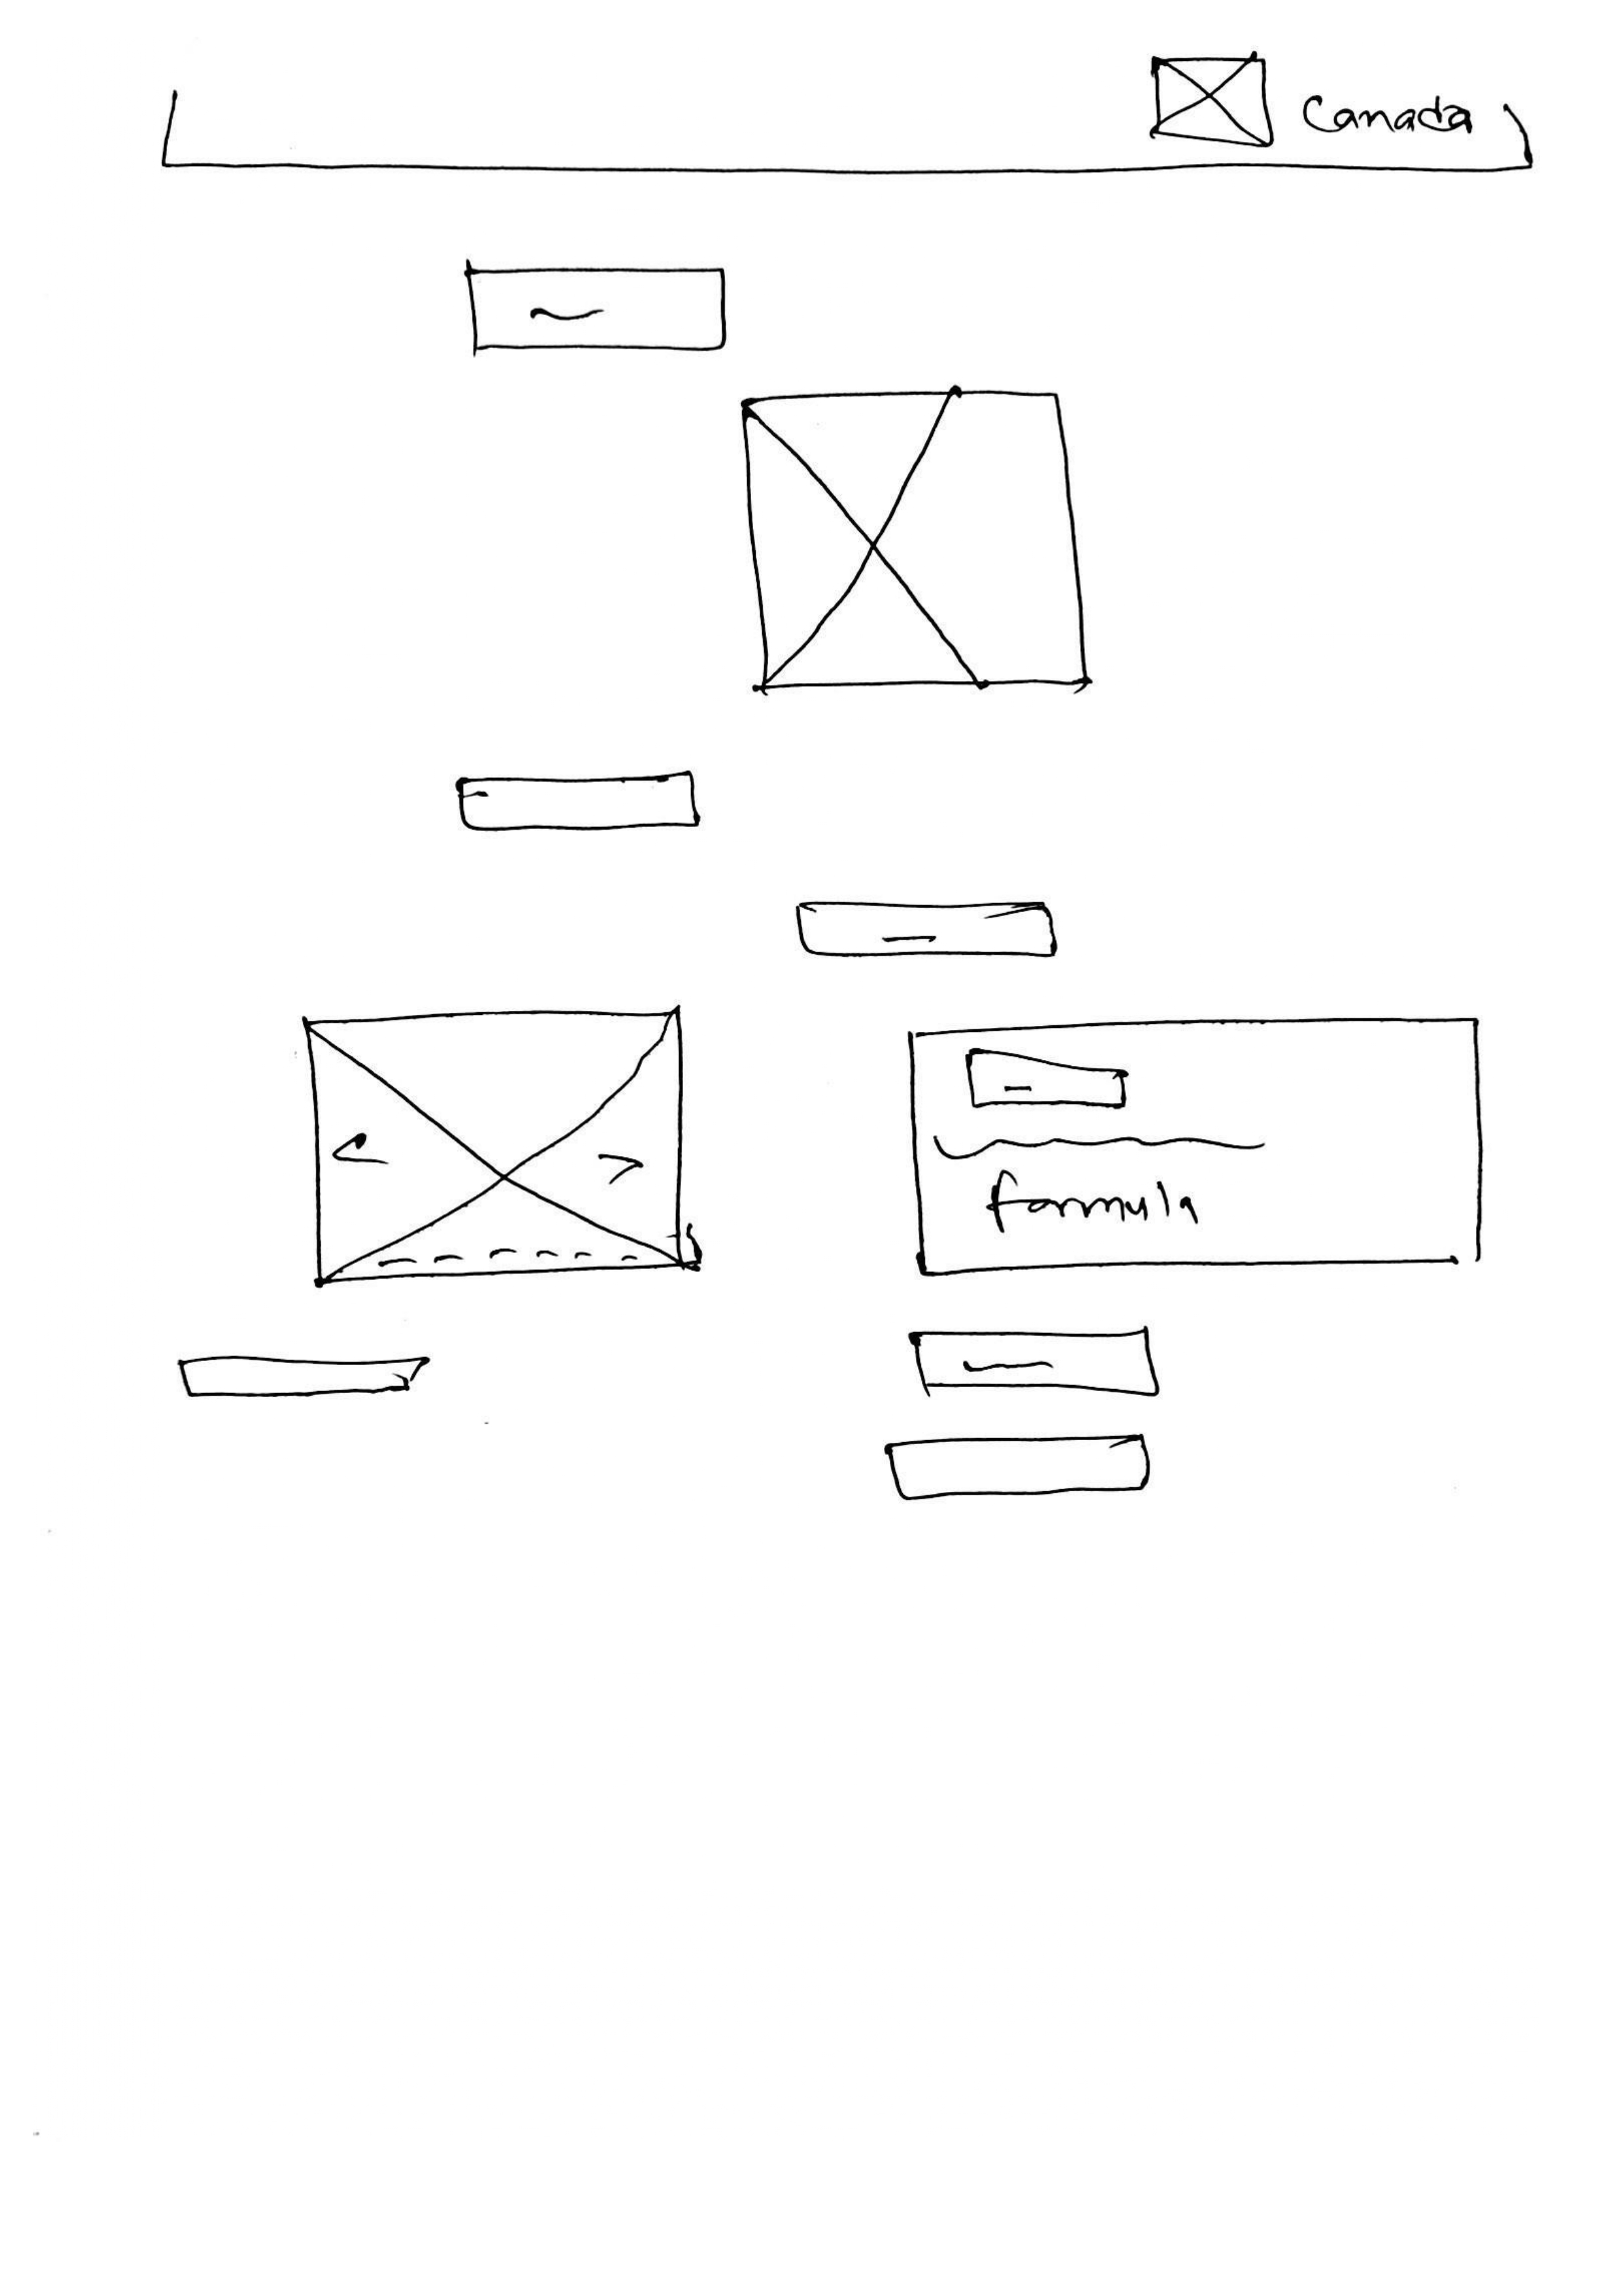
\includegraphics[scale=.6, trim=30 300 0 0 ]{images/si2.jpg}
        \caption{Sample Input Image}
        \label{fig:lsam1}
    \end{figure}


The sample \gls{dsl} for above image:

% Use the custom command to display the tree structure

\begin{verbatim}
    header{
        flex{
            logodiv{
                image
            }
            nav{
                navlink
                navlink
                navlink
                navlink
                navlink
            }
        }
    }
    \end{verbatim}

    
    \subsubsection{Customization}  
    In this project, simply converting the sketch into HTML code is not enough to create a fully functional web page. While the sketch serves as a basic framework for the layout, it is still lacking essential details such as color schemes, fonts, and other styles. The sketch represents only a rough blueprint of the web page, providing the basic positions of elements but not offering any visual appeal or design choices. To make the final result visually pleasing and user-friendly, the various components on the web page must be styled correctly. Styling not only includes the layout but also focuses on how different elements such as buttons, text, images, and containers appear to the user. 
    This project, therefore, allows for extensive customization options so that the user can personalize the design to their liking. It enables theme selection, where users can choose from a variety of pre-defined themes that reflect different aesthetic styles. These themes determine how the web page will look in terms of color combinations, background designs, and overall visual appeal. Additionally, users have the flexibility to select a color palette that suits their preferences or the brand's color identity. The ability to pick from a range of font styles ensures that the typography aligns with the intended tone and purpose of the web page. Whether it’s for a formal business website or a fun and casual blog, the font selection is key in setting the right mood for the page.
    Apart from theme selection, users can further refine the design by customizing the individual styles of various elements on the page. This includes choosing specific fonts, adjusting font sizes, altering text alignments, and picking colors for headers, paragraphs, buttons, and links. Users can even go as far as deciding how elements like navigation bars, footers, and images should behave and appear on different screen sizes.
    When it comes to text content, this project will provide randomly generated placeholder text, often referred to as "Lorem Ipsum," which serves as a stand-in for the actual content that the user will later customize. This generated text helps visualize the page layout and provides a placeholder for where the content will go, but users can replace it with their own text at any time. This flexibility allows users to quickly visualize the layout with sample content while giving them the freedom to change it when the real text is available.
    For images, placeholders are used initially to represent where images will be placed within the design. The user has the option to either provide an image link from the web or upload images directly from their computer. The placeholder image can be replaced easily, allowing users to try out different visuals or insert their own brand images to personalize the page.
    In summary, this project provides extensive customization options, enabling users to create unique and visually appealing web pages based on their specific requirements. Whether it’s choosing a theme, adjusting fonts, altering colors, or adding images and content, the customization feature gives users complete control over the final appearance and design of the web page, making it a flexible and versatile tool for web development.
    
    \subsubsection{Compiler}  
    A compiler is a specialized computer program responsible for translating code written in one programming language into another programming language. In our case, the compiler takes the Domain-Specific Language (DSL) that we have created and translates it into HTML and CSS code, which are the standard languages used to design and structure web pages. 
    The role of the compiler is crucial because it bridges the gap between the abstract design defined in DSL and the practical web page that can be viewed in a browser. Our compiler is designed to read a mapping file written in JSON format. This file contains instructions that tell the compiler how each DSL token should be converted into corresponding HTML tags, which are then used to create the structure of the web page. By processing the input DSL code, the compiler produces a structured HTML document, while also applying relevant styles using CSS.
    The compiler reads these mapping instructions from a JSON file, which acts as an intermediary format that combines both the structural blueprint of the page and the dynamic content provided by the user. This JSON file contains all the necessary data to transform the DSL elements into a fully functional page, complete with user-specific content.
    Once the JSON file has been generated, the compiler proceeds to convert it into HTML and CSS. The HTML structure is generated based on the hierarchy and relationships defined in the DSL, ensuring that the content is displayed correctly. The CSS, on the other hand, applies styling to the HTML elements, ensuring that the web page looks visually appealing. This process includes applying dynamic variables, such as colors, font choices, and layout styles, which have been selected by the user during the customization phase.
    The final output is a complete, functional web page that is fully styled and ready to be viewed in a browser. The compiler ensures that the web page retains the structure defined in the DSL, while also integrating the user’s content and styling choices. This seamless translation from DSL to HTML and CSS enables users to quickly create customized web pages without the need for manual coding, streamlining the entire development process.
    In conclusion, the compiler plays a vital role in transforming the abstract design and structure defined by the user in DSL into a fully functional web page. By converting the DSL code into HTML and CSS, the compiler not only generates the necessary content but also ensures that the web page is visually appealing and responsive. With the ability to handle multiple platforms, the compiler offers a versatile solution for creating web pages that can be used across different devices and environments.

\subsection{Activation Function}
Activation functions play an essential role in neural networks by determining the output of each neuron or unit in the network. They are mathematical functions that take in input values (the weighted sum of the previous layer’s outputs) and apply a transformation to decide the neuron’s output. Without activation functions, the neural network would essentially be just a linear regression model, regardless of the number of layers. This is because, when combined, two linear functions still result in a linear function. This limits the ability of the network to learn complex patterns in data, which is why non-linear activation functions are necessary.
The purpose of the activation function is to introduce non-linearity into the network. Non-linear functions enable the network to learn from the data more effectively by allowing it to model complex relationships between inputs and outputs. This is crucial because real-world data is often non-linear, and a linear function would not capture the complex relationships that exist in tasks such as image recognition, language translation, or prediction.
In this project, the use of specific activation functions helps the neural network to learn and generalize better. Different types of activation functions are used at various layers within the network, and they serve different purposes depending on the architecture and type of network being used. Some functions work better in the hidden layers, while others are more suitable for the output layer.
\subsubsection{Softmax Function}
The Softmax function is sometimes called the soft argmax function, or multi-class
logistic regression since it is a generalization of logistic regression that can be used for
11 multi-class classification. The softmax function is ideally used in the output layer of the classifier where the probabilities are required to define the input images’ class. A
softmax function calculates the probabilities of each class which the input belongs. The
softmax units in the output layer always be equal to number of classes. The probability
distribution is different for different classes and the summation value of all probability
distribution is 1. The softmax function 4.4 provides the probability values for each
classes and class with highest probability value is consider as correct prediction.


\begin{equation}
\text{softmax}\sigma(\vec{z})_i = \frac{e^{z_i}}{\sum_{j} e^{z_j}}
\end{equation}
Where
\begin{align*}
    z_i &: \text{ elements of the input vector,} \\
    e^{z_i} &: \text{ standard exponential function applied to each element,} \\
    K &: \text{ number of classes in the multi-class classifier.}
\end{align*}\quad



The Softmax function is a function that turns a vector of K real values into a vector of
K real values that sum to 1. The input values can be positive, negative, zero, or greater
than one, but the values are converted to values between 0 and 1 by softmax. Thus now
they are interpreted as probability. Small or negative inputs are converted to a small
probability value.

\subsubsection{ReLU Function}
\gls{relu} is one of the most widely used activation functions in deep learning and neural networks. It has become a go-to choice due to its simplicity and effectiveness. The \gls{relu} function works by applying a transformation to the input data, where it outputs zero for all negative input values and outputs the input value itself if it is positive. The mathematical equation for the \gls{relu} activation function is:



\begin{equation}
\text{ReLU}(x) = \max(0, x)
\end{equation}
This equation means that if the input,x, is greater than zero, then the output is x. However, if 
x is less than or equal to zero, the output becomes zero.

\begin{equation}
\frac{d}{dx} \text{ReLU}(x) = 
\begin{cases} 
0 & \text{if } x \leq 0 \\
1 & \text{if } x > 0
\end{cases}
\end{equation}

\begin{figure}[H]
    \centering
    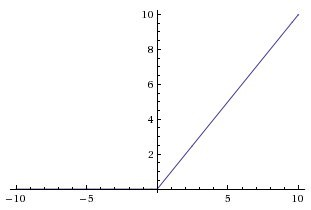
\includegraphics[scale=1]{images/RELU.jpg}
    \caption{Graphical Representation of ReLU Function}
    \label{fig:relu-}
\end{figure}



\subsection{Loss Function and Optimizer}
In machine learning, the loss function and optimizer are integral to the learning process. These components directly influence how a model learns from data, improves its performance, and ultimately makes accurate predictions. The loss function is a mathematical formula that calculates the error between the predicted output of the model and the actual target values. In other words, it quantifies how well or poorly the model is performing. The objective during training is to minimize this loss, effectively improving the model's ability to make accurate predictions. Different types of loss functions are used depending on the type of problem such as classification, regression, or generative tasks. In this project, the loss function will guide the model to generate accurate HTML code from sketch input by minimizing the discrepancies between predicted and actual HTML structures.
Once the loss function has been calculated, the optimizer steps in. An optimizer’s primary role is to update the model’s weights (parameters) in a way that minimizes the loss function. This is done by calculating the gradients, which indicate the direction and magnitude of changes required to reduce the loss. The optimizer adjusts the weights incrementally to steer the model toward a more accurate solution. One of the key aspects of the optimizer is how it controls the learning rate a parameter that determines the size of each step. A proper learning rate is critical to ensure the model does not overshoot the optimal solution or get stuck in a suboptimal one. For the task of converting sketches to HTML code in this project, the optimizer helps fine-tune the parameters, ensuring that the model learns from the sketches efficiently and generates precise code.
The combination of a well-chosen loss function and an effective optimizer is fundamental to successful model training. While the loss function guides the model by highlighting the areas where improvement is needed, the optimizer ensures that those improvements are made in the most effective manner possible. Together, they enable the model to learn not just from data but in the way that is most appropriate for generating HTML code from sketches in our project.
\subsubsection{Categorical Cross-Entropy}
Categorical cross-entropy is one of the most widely used loss functions in machine learning, especially in classification problems where the model is tasked with predicting a class label from multiple possible categories. This function is particularly useful in scenarios where the output involves a probability distribution over different classes, such as in multi-class classification problems. The categorical cross-entropy loss quantifies the difference between the predicted probability distribution and the true distribution, or target values. It does this by penalizing the model more when it assigns higher probabilities to incorrect classes and less when it assigns higher probabilities to correct classes. This helps the model learn to make more accurate predictions over time.
The formula for calculating categorical cross-entropy is as follows:
\begin{equation}
\text{Loss} = -\sum_{i=1}^{\text{Output size}} y_i \log(\hat{y}_i)
\end{equation}

Where:
\begin{itemize}
    \item \(\hat{y}_i\) is the predicted probability of the \(i\)th class, as output by the model.
    \item \(y_i\) is the true value (or target) for the \(i\)th class. This is typically represented as a one-hot encoded vector, where the correct class is marked with a 1 and all others are 0.
    \item The output size refers to the total number of classes the model is predicting over (the size of the output vector).
\end{itemize}
In the context of this project, where we aim to predict HTML structures from sketches, categorical cross-entropy would be applied to measure how well the model’s output (the predicted HTML tags and structures) matches the target HTML output. By minimizing this loss function, the model learns to improve its predictions over time, eventually generating HTML code that is structurally and syntactically correct, based on the input sketch. The use of categorical cross-entropy is crucial for ensuring that the model's predictions are accurate in a multi-class setting, where each class corresponds to a different HTML element or attribute.

\subsubsection{Adam Optimizer}

The Adam optimizer, which stands for Adaptive Moment Estimation, is one of the most widely used optimization algorithms in the training of deep learning models. It combines the advantages of two other popular optimization techniques: AdaGrad and RMSProp. Adam computes adaptive learning rates for each parameter by maintaining two moving averages: the first moment \(m\) (which represents the mean of the gradients) and the second moment \(v\) (which represents the uncentered variance of the gradients). These moving averages are used to adjust the learning rates of the model's parameters in a more informed and dynamic way during training.
The key advantage of Adam lies in its ability to adaptively adjust the learning rates for each parameter based on the gradients' first and second moments. This means that parameters associated with larger gradients receive a lower learning rate, while parameters with smaller gradients are updated more aggressively. This adaptive approach helps accelerate convergence, particularly in problems involving sparse gradients or noisy data. Moreover, Adam is designed to work well with non-stationary objectives, making it highly effective in real-world applications where data may change or evolve over time.

The optimization process in Adam involves the following steps:
\begin{itemize}
    \item Compute the gradient of the loss function with respect to the model parameters.
    \item Update the first moment estimate (\(m\)) as the exponential moving average of the gradient.
    \item Update the second moment estimate (\(v\)) as the exponential moving average of the squared gradient.
    \item Compute a bias-corrected estimate of the first and second moments to counteract initialization bias.
    \item Adjust the learning rate for each parameter based on the moving averages of the gradients and their variances.
    \item Update the model parameters using these adjusted learning rates.
\end{itemize}

Adam has gained popularity due to its simplicity of implementation, computational efficiency, and low memory requirements. It does not require a lot of hyperparameter tuning, making it user-friendly for both beginners and experienced practitioners. Additionally, Adam is invariant to diagonal rescaling of the gradients, meaning that it is robust to changes in the scale of the input data, a property that makes it suitable for a wide range of deep learning tasks.
In the context of this project, where the task involves generating HTML structures from input sketches, Adam provides an efficient way to train the model while adapting the learning rates based on the gradients of the loss function. Its ability to handle large datasets, combined with the adaptive learning rate mechanism, helps the model converge faster and achieve better performance. By using Adam, we ensure that our model is both computationally efficient and capable of adapting to the complexities of the task at hand.


\subsection{Performance Metrics}
In machine learning, performance metrics are essential for evaluating how well a model performs on a given task. These metrics offer quantitative measures of a model's accuracy and reliability, guiding the development process by helping to determine whether the model is underfitting, overfitting, or generalizing well to new data. For text generation tasks, such as generating HTML from sketches, using appropriate metrics is crucial to assess the quality and relevance of the generated content compared to the expected output.
For this project, we utilize two popular performance metrics—BLEU (Bilingual Evaluation Understudy) and ROUGE (Recall-Oriented Understudy for Gisting Evaluation)—to evaluate the model's effectiveness. Both of these metrics are commonly used in natural language processing (NLP) tasks, especially in machine translation and text summarization, but they can also be applied to evaluate the quality of generated text in our use case.
\subsubsection{BLEU}
\gls{bleu} is an algorithm for evaluating the quality of
text which has been machine-translated from one natural language to another. This is
a common metric used in machine translation tasks, which seeks to measure how
closely a machine-generated text resembles what a human would have generated, given
the same input. It is based on n-gram based precision. Four sub metrics are denotes as
BLEUn, for n = 1, 2, 3, 4. For a candidate sentence a and a set of reference sentences
b, the BLEU score is calculated as:
\begin{equation}
\text{BLEU}_n(a, b) = \frac{\sum_{w_n \in a} \min\left(\text{count}_a(w_n), \max_{j=1, \ldots, |b|} \text{count}_{b_j}(w_n)\right)}{\sum_{w_n \in a} \text{count}_a(w_n)}
\end{equation}
where wn denotes n-gram, counta(wn) denotes count of n-gram wn in sentence
\subsubsection{ROUGE}
ROUGE (Recall-Oriented Understudy for Gisting Evaluation) is an evaluation metric
specially designed for automatic summarization that can be used for machine
translation. It measures the overlap of n-grams between the generated sequence and
reference sequence. The ROUGE score is calculated as:
\begin{equation}
\text{ROUGE-N Precision} = \frac{\sum_{n}\text{count}_{\text{match}}(n)}{\sum_{n}\text{count}_{\text{generated}}(n)}
\end{equation}
\begin{equation}
\text{ROUGE-N Recall} = \frac{\sum_{n}\text{count}_{\text{match}}(n)}{\sum_{n}\text{count}_{\text{reference}}(n)}
\end{equation}
\begin{equation}
\text{ROUGE-N F1} = \frac{2 \times \text{ROUGE-N Precision} \times \text{ROUGE-N Recall}}{\text{ROUGE-N Precision} + \text{ROUGE-N Recall}}
\end{equation}





\subsection{Flowchart}
\subsubsection{During Training}
\begin{figure}[H]
    \centering
    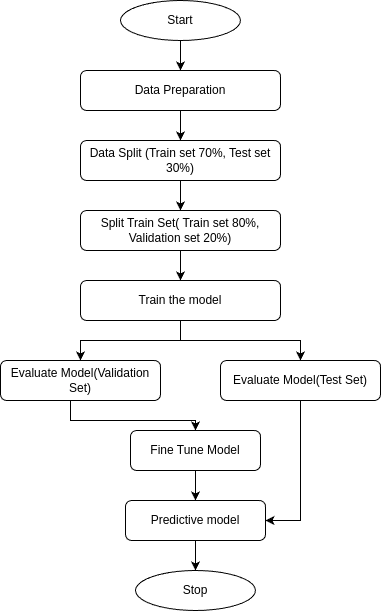
\includegraphics[scale=0.8]{images/training flowchart.png}
    \caption{Training Flowchart}
    \label{fig:flowtra}
\end{figure}

\subsubsection{During Testing}
 \begin{figure}[H]
 \centering
        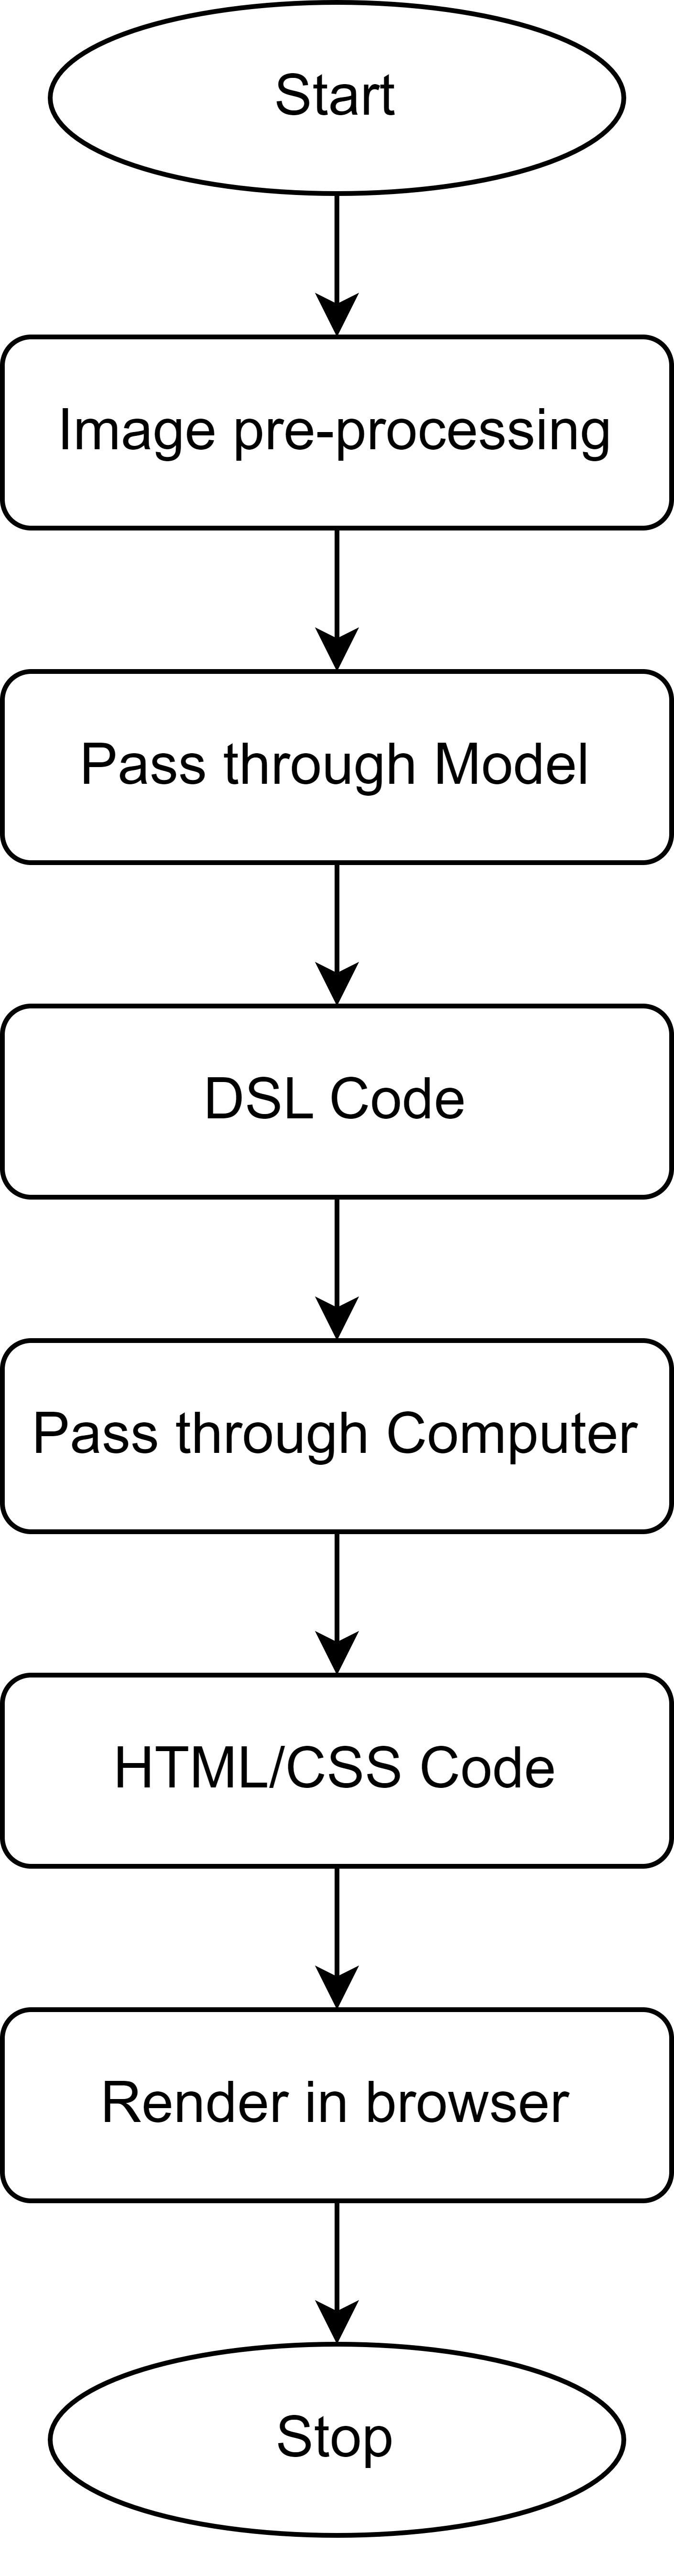
\includegraphics[scale=1.5]{images/testing flowchart.png}
        \caption{Testing Flowchart}
        \label{fig:flowtr}
    \end{figure}




    \pagebreak